\section{Tests et bugs}

\subsection{Interface}

Pour la partie interface, nous avons essayé de simuler une exécution de génération de ville, en commençant par le bouton "générer une ville aléatoire" puis "paramétrer sa ville":

\begin{itemize}
	\item Générer une ville aléatoirement : Lorsqu'on appuie sur le bouton avec un ordinateur qui a la même configuration que celui utilisé pour l'analyse de l'existant, la génération de ville se fait en 10 secondes, ce qui est bien loin de ce que l'on espérait au début soit être à environ 24 000 bâtiments en 3,5 secondes comme Citygen.
	\item Paramétrer sa ville : Le bouton "paramétrer sa ville" donne accès à une nouvelle fenêtre dans laquelle il est possible de trziter la taille de la ville et si l'on veut une rivière ou non. L'affichage de la nouvelle page se fait correctement et rapidement, seulement les deux boutons affichés par la suite ne fonctionne pas, on est obligé de quitter la génération si l'on veut retourner à la page d'accueil.
\end{itemize}

\subsection{Terrain}

Pour le terrain nous avons testé les limites que celui-ci apporte, par exemple en augmentant à la limite du possible le maillage du terrain, ainsi que moduler les paramètres du bruit de Perlin pour voir si on obtient des bugs ou non.

\begin{itemize}
	\item Maillage : Lorsque l'on utilise un maillage inférieur ou égal à 250 par 250, l'affichage du terrain se fait correctement, nous n'avons pas d'erreur d'affichage et le terrain est correct.
\end{itemize}
	
\begin{center}
	\centering
    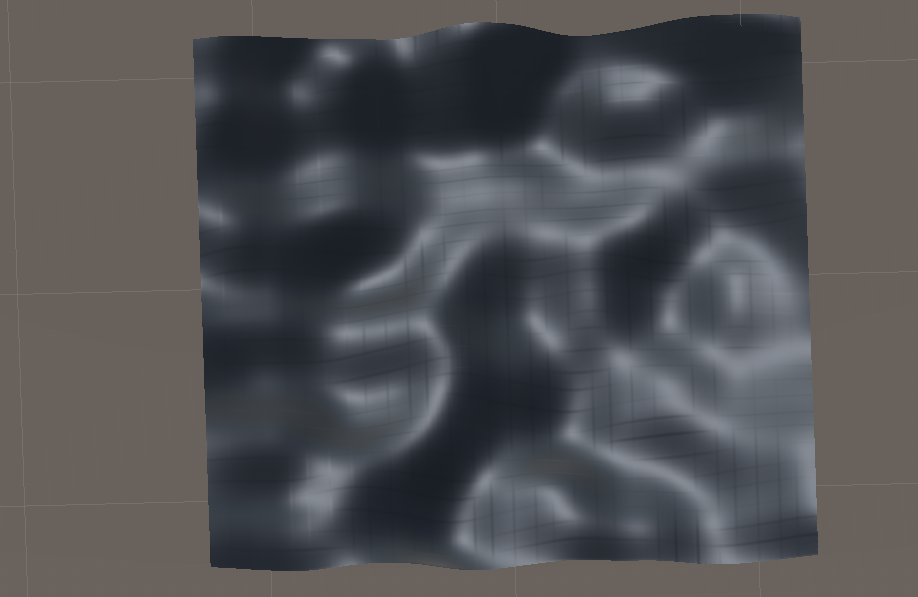
\includegraphics[height = 5 cm]{images/maille(250x250).png}\\
	 \captionof{figure}\small{Maille 250x250}
\end{center}

	Cependant lorsque l'on met en place des paramètres au-delà de cette valeur, on obtient un bruit de Perlin qui n'est pas correct car on y apperçoit des lignes, comme si la zone avait été saturée par la trop forte quantité de maillage.
	
\begin{center}
	\centering
    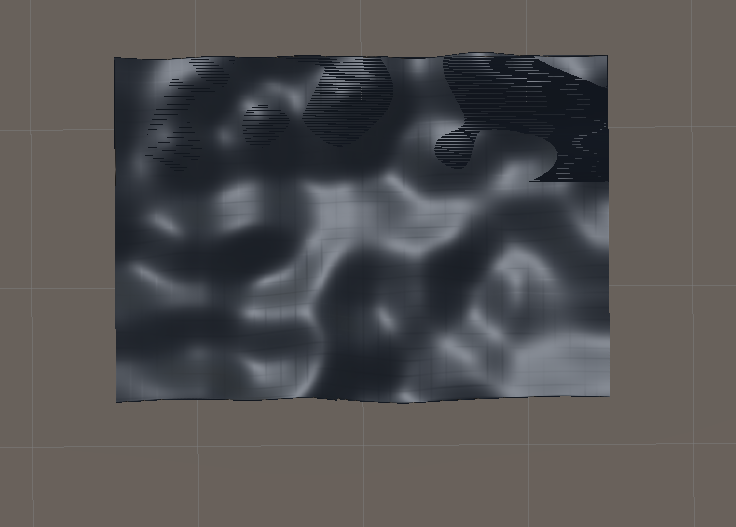
\includegraphics[height = 5 cm]{images/maille(350x350).png}\\
	 \captionof{figure}\small{Maille 350x350}
\end{center}

\begin{itemize}
	\item Bruit de Perlin : Lorsque l'on change les paramètres sur la hauteur des coordonnées et qu'on les mets à l'extrême, on obtient un terrain correct, seulement il est impossible de l'utiliser car les ondulations sont beaucoup trop conséquentes. À l'inverse si l'on met tout au minimum, on obtient un terrain plat sans bugs.
	
	\item Fusion terrain et ville : nous n'avions pas clairement réussi à fusionner le terrain et la ville lors de la génération, même si les deux éléments existe distinctement et que l'on peut mettre une ville à la main sur le terrain. Ce problème a été solutionner en mettant en place un creux sur le terrain pour mettre une partie du terrain à hauteur zéro et y placer la ville.
\end{itemize}

\subsection{Ville}

Pour tester la génération de ville nous avons mis en place un test de limite qui considère dans un premier temps le comportement d'une petite ville (citysize : 50) et celui d'une plus grande ville (citysize : 600).

\begin{itemize}
	\item Petite ville : L'exécution de la petite ville se fait assez rapidement, cependant au niveau de l'affichage on recontre quelques problèmes, les éléments de la ville sont à l'extérieur de la muraille (on observe ce phénomène également sur une plus grande ville mais moins fréquemment), il est donc impossible d'avoir une ville correcte si on veut qu'elle soit petite.
	
\begin{center}
	\centering
    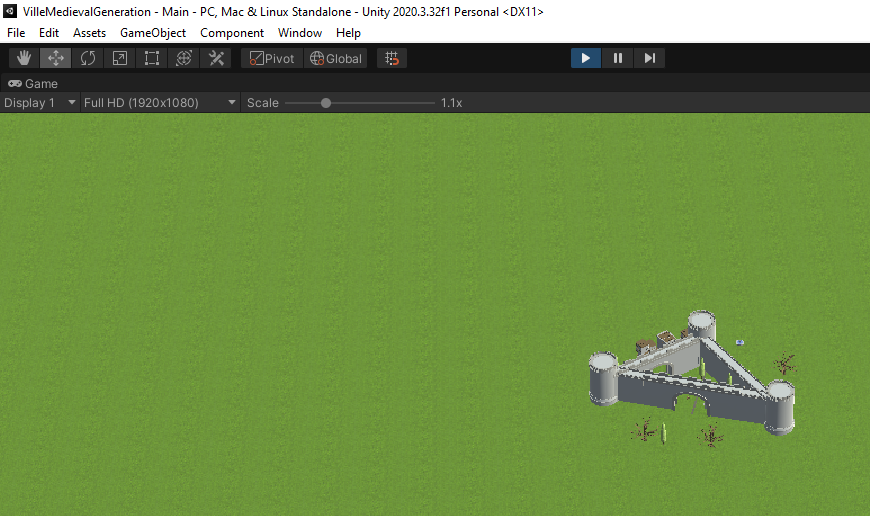
\includegraphics[height = 5 cm]{images/testville.png}\\
	\captionof{figure}\small{Ville de taille 50}
\end{center}

	\item Grande ville : L'exécution de la grande ville est un peu plus fastidieux en terme de temps et d'affichage, nous avons réussi au maximum à créer une ville de taille 600 qui met 30 secondes à se générer, au delà de cette taille l'affichage est impossible que le pc crash avant de pouvoir finir la génération. Nous remarquons que dans ce cas précis de grande ville nous n'avons pas de bug de bâtiments en dehors de la muraille, donc il est possible que le bug de la muraille dépendent de la taille de la ville.
	
\begin{center}
	\centering
    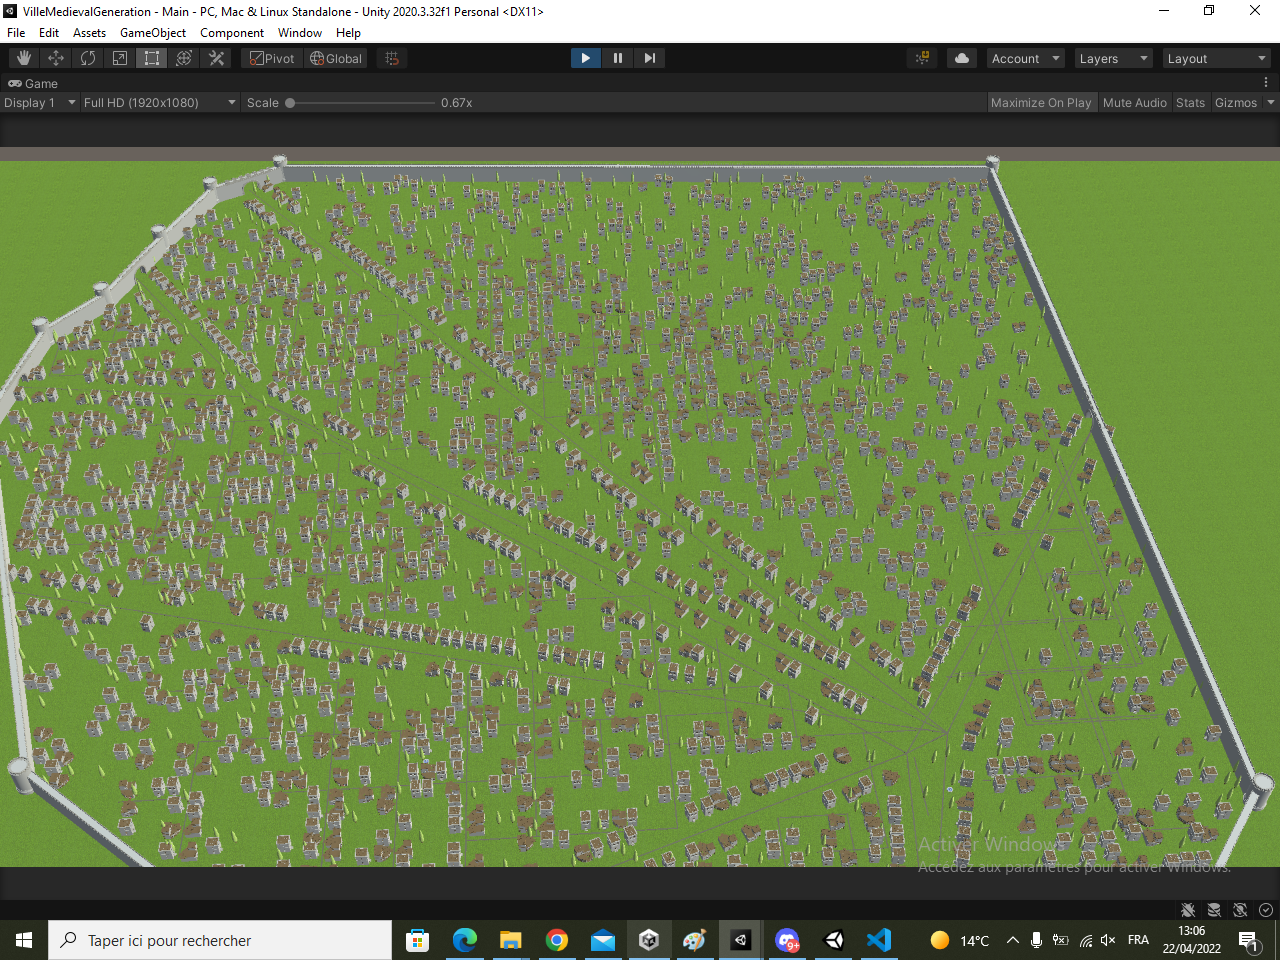
\includegraphics[height = 5 cm]{images/testville2.png}\\
	\captionof{figure}\small{Ville de taille 50}
\end{center}

	\item Ville avec terrain : il arrive aussi que la ville ne se mette pas directement en lien avec le terrain, les murailles débordent, et le bug sur les bâtiments qui dépassent de la muraille est aussi fréquent. 
	
	
\begin{center}
	\centering
    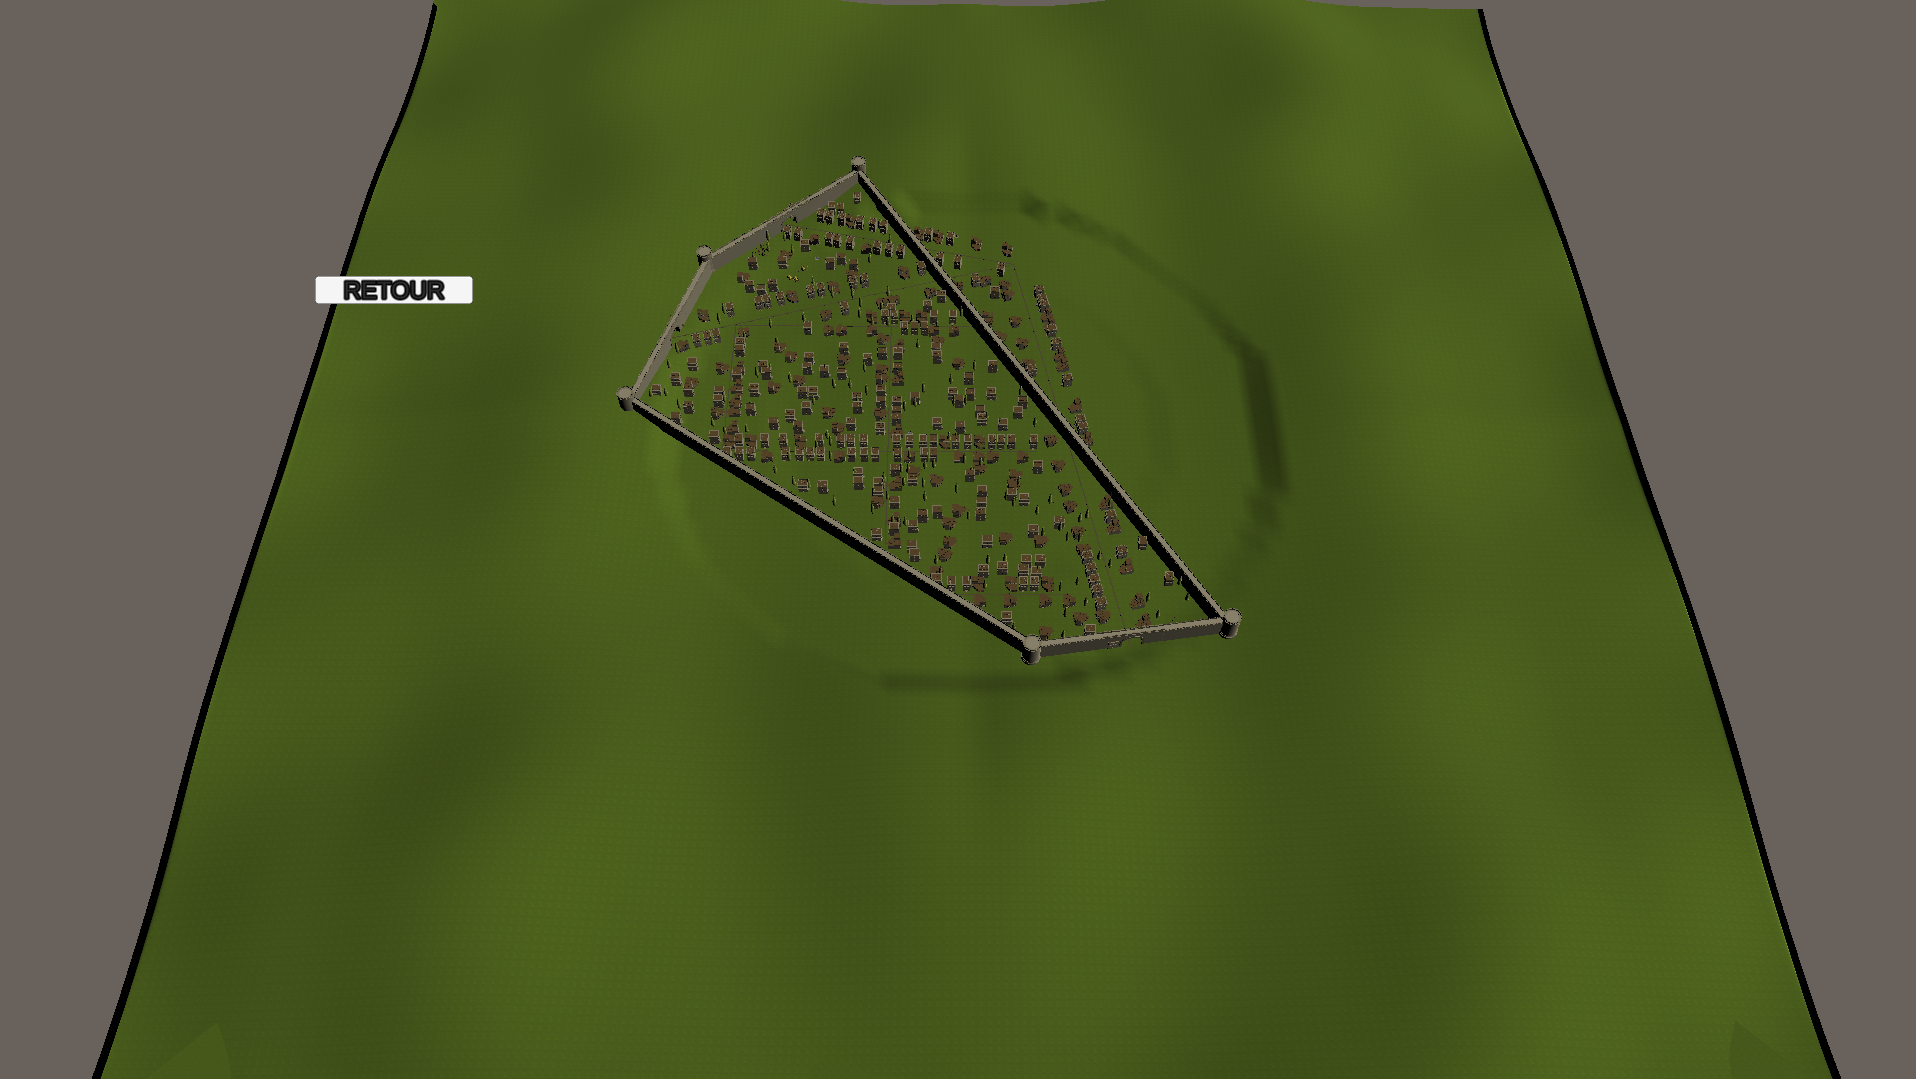
\includegraphics[height = 5 cm]{images/testville3.png}\\
	\captionof{figure}\small{Ville avec terrain}
\end{center}
	
\end{itemize}

Nous avions également rencontré des bugs sur la générations des terrains qui ne se faisait pas autour des routes mais nous avons solutionner le problème, également sur les L-system qui ont créé des routes similaires à la création de plusieurs branches qui se croisaient, nous avons réglé le problème en créant des routes qui sont plus rectangulaires. Également si nous mettons en place plusieurs routes principales, nous ne recontrons pas de bug (à la limite du lisible) et chaque route principales sort par une porte de la muraille.